% =====================================================================
%  Dusk Park (黃昏樂園) — Computer Graphics Final Project Design Document
%  Built with Tectonic.  Pure English.
% =====================================================================
\documentclass[11pt,a4paper]{article}

% ---------- Packages ----------
\usepackage[margin=1in]{geometry}
\usepackage[utf8]{inputenc}
\usepackage[T1]{fontenc}
\usepackage{lmodern}
\usepackage{microtype}
\usepackage{graphicx}
\usepackage{xcolor}
\usepackage{enumitem}
\usepackage{booktabs}
\usepackage{tabularx}
\usepackage{titlesec}
\usepackage{parskip}
\usepackage[hidelinks]{hyperref}
\usepackage{fontspec}
\usepackage{xeCJK}
\setCJKmainfont{Noto Serif CJK TC}
\usepackage{amsmath}
\usepackage{float}
\usepackage{caption}
\usepackage{listings}

% ---------- Colour helpers ----------
\definecolor{duskorange}{HTML}{FF7A35}
\definecolor{duskpurple}{HTML}{3A1655}
\definecolor{neoncyan}{HTML}{4DDEF0}
\definecolor{neonpink}{HTML}{FF4D99}
\definecolor{codebg}{HTML}{F7F4EF}

% ---------- Section style ----------
\titleformat{\section}{\normalfont\Large\bfseries\color{duskpurple}}{\thesection}{0.7em}{}
\titleformat{\subsection}{\normalfont\large\bfseries\color{duskorange!80!black}}{\thesubsection}{0.7em}{}

% ---------- Listings ----------
\lstset{
  basicstyle=\ttfamily\footnotesize,
  backgroundcolor=\color{codebg},
  frame=single,
  framerule=0pt,
  rulecolor=\color{codebg},
  xleftmargin=8pt,
  xrightmargin=4pt,
  aboveskip=6pt,
  belowskip=6pt,
  breaklines=true,
  columns=fullflexible,
}

% ---------- Student info ----------
\newcommand{\studentid}[0]{41173058H}
\newcommand{\studentname}[0]{鍾詠傑 (Chung Yung-Chieh)}

\begin{document}

% =====================================================================
\section*{Dusk Park --- Design Document}
\addcontentsline{toc}{section}{Dusk Park --- Design Document}

\noindent\textbf{Live demo:} \url{https://g36maid.github.io/cg-final-project/Theme-Park/}

\begin{tabularx}{\textwidth}{@{}lX@{}}
  \textbf{Student ID:}  & \studentid \\
  \textbf{Name:}        & \studentname \\
\end{tabularx}

\vspace{4pt}

\begin{figure}[H]
  \centering
  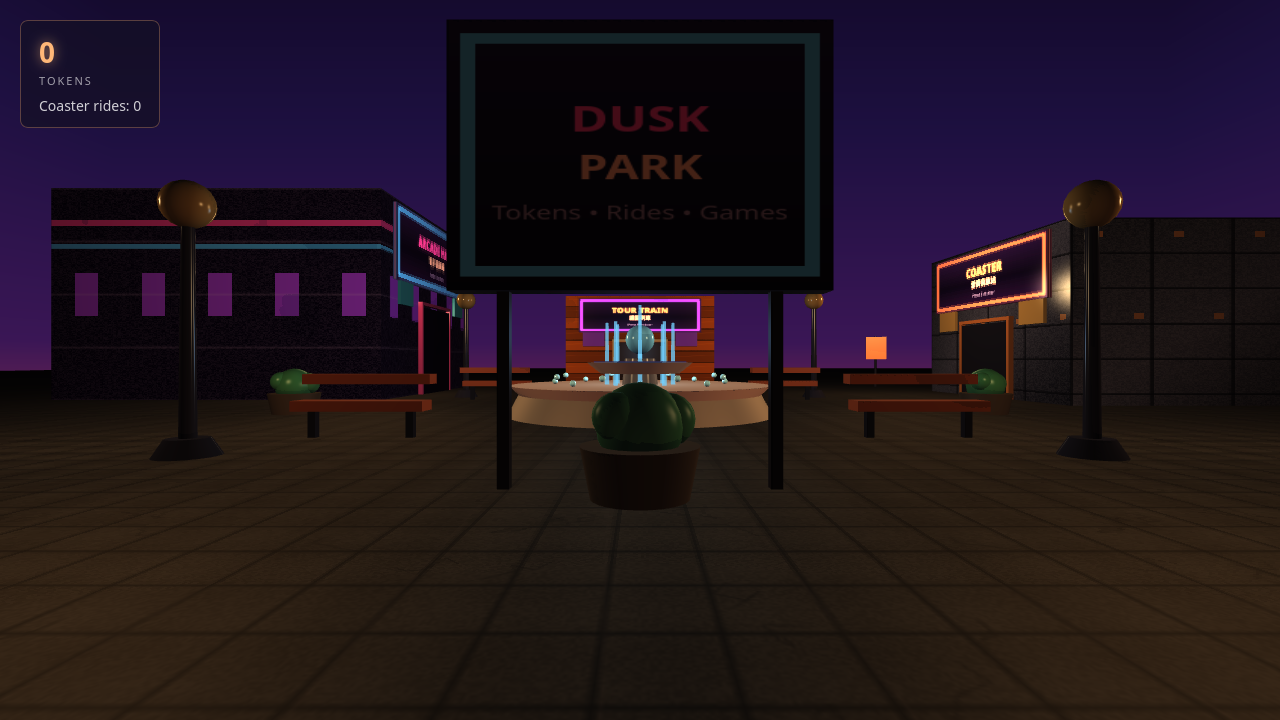
\includegraphics[width=\textwidth]{figures/theme-park-hub.png}
  \caption{The Dusk Park hub at golden hour. The player stands in the central plaza with the
  reflecting fountain (T6), procedurally textured buildings, warm lamp point lights (T3), the
  dusk-gradient skybox (T5), and long dramatic shadows cast by the directional sun (T7).}
  \label{fig:hub}
\end{figure}

\tableofcontents
\vspace{4pt}

% =====================================================================
\section{Game Concept}

\textbf{Dusk Park} is a 3D theme-park meta-game. The player wanders an outdoor plaza at
dusk and visits four integrated sub-games: a neon \emph{Pinball} table, a \emph{Rubik's
Cube} solver, a \emph{3D Tetris} well, and a \emph{Roller Coaster} ride. Three of these
sub-games (Pinball, Rubik's Cube, Tetris) are arcade machines that \emph{award} tokens on
completion; the Roller Coaster \emph{consumes} tokens per ride. The meta-objective is
simple and clearly communicated to the player through the HUD and an information board:

\begin{quote}
  \textit{Earn tokens by playing arcade games, then spend them on coaster rides.
  After three rides the tour is ``complete'' and a fireworks celebration plays.}
\end{quote}

The hub itself is a first-person walkthrough scene that concentrates every hard graphics
requirement of the course spec (T1--T7): player movement, first/third-person camera, Phong
point lights, textured surfaces, a skybox cubemap, cubemap reflection on the fountain
water, and shadow mapping. The sub-games are integrated through page navigation and
\texttt{localStorage}-based token persistence, so each sub-game keeps its own renderer and
gameplay intact.

The experience we want the player to have is one of \emph{wandering a park caught between
day and night}. Dusk is the narrative metaphor: the park sits at the boundary of reality
(the hub) and the game universes behind each door, and the warm light makes every graphics
technique read clearly on screen.

% =====================================================================
\section{Scene \& Visual Design}

\subsection{Why Dusk?}

We deliberately rejected both daytime and night. Under a daytime sky the point-light
contribution is visually negligible (sun washes it out) and shadows are short and flat; at
night the coaster landscape is invisible and the arcade exteriors lose their context.
\textbf{Dusk} is the single time of day where every required technique is simultaneously
visible and dramatic:

\begin{itemize}[nosep]
  \item \textbf{Point lights + Phong} --- the low ambient lets the warm lamp lights and
    their ambient/diffuse/specular components all read on the dark building facades.
  \item \textbf{Shadows} --- the low sun angle stretches building shadows across the plaza,
    making the shadow map obvious rather than subtle.
  \item \textbf{Skybox} --- the orange-to-purple dusk gradient is visually richer than a
    flat blue day sky and is cheap to generate procedurally.
  \item \textbf{Reflection} --- the fountain water reflects the colourful sky and neon
    signs, which is far more legible than reflecting a uniform blue daytime sky.
\end{itemize}

\subsection{Colour Palette}

The palette (Table~\ref{tab:palette}) is built around a warm-cool tension: warm
orange/gold for the sun and lamps, cool purple/indigo for the sky and ambient, and
saturated neon pink/cyan as accents that bridge the hub to the arcade interiors.

\begin{table}[H]
  \centering
  \caption{Key colours and their roles.}
  \label{tab:palette}
  \begin{tabularx}{\textwidth}{@{}llX@{}}
    \toprule
    \textbf{Role} & \textbf{Hex} & \textbf{Purpose} \\
    \midrule
    Sky zenith     & \texttt{\#0A0418} & Deep indigo, anchors the top of the cubemap \\
    Sky horizon    & \texttt{\#FF7A35} & Warm sunset band where the eye is drawn \\
    Ambient        & \texttt{\#1F1A2E} & Cool purple fill, matches the sky's cool side \\
    Sun (fill)     & \texttt{\#FFA65E} & Low-angle directional light at intensity 0.35 \\
    Lamp (point)   & \texttt{\#FFD98C} & Warm yellow point lights at intensity 1.8 \\
    Neon pink      & \texttt{\#FF4D99} & Arcade hall accent, banners \\
    Neon cyan      & \texttt{\#4DDEF0} & Signage borders, fountain sparkles \\
    Stone ground   & \texttt{\#59504A} & Neutral absorptive surface; takes shadows well \\
    \bottomrule
  \end{tabularx}
\end{table}

\subsection{Objects in the Scene}

The plaza contains three landmark buildings, a central fountain, an information board,
street lamps, benches, planters, and decorative banners. Each major object earns its place:
the \textbf{Arcade Hall} (neon-striped facade) is the portal to the three arcade
sub-games; the \textbf{Coaster Station} (metal grid facade) gates the token-gated ride;
the \textbf{Tour Train} station (wooden planks) anchors the far end of the plaza. The
\textbf{central fountain} is the showcase for cubemap reflection (T6) and sits at the
visual centre so the player encounters it immediately. The \textbf{information board} at
the entrance provides the in-game instructions (D6).

% =====================================================================
\section{Technical Choices}

\subsection{Camera \& Projection}

The camera uses a perspective projection with a \textbf{65\textdegree{} FOV}. We chose a
slightly wider-than-default FOV because the park is an open plaza the player must take in
laterally; a narrow FOV would feel tunnel-visioned when standing among the buildings. The
\textbf{near plane is 0.1} and the \textbf{far plane is 1000}; the large far plane is
required because the skybox box is $500^3$ units and must never be clipped. The canvas
fills the browser viewport (16:9 in the screenshot), so the aspect ratio matches the
display.

In first person the camera sits at the player's \textbf{eye height of 1.7 units}, a
deliberately human scale so the buildings (7--9 units tall) tower over the player and the
fountain (2.3-unit orb) is at a comfortable viewing angle. Pressing \texttt{C} switches to
a third-person view that pulls the camera 6 units back and 3 units up; this exists to
satisfy the spec's ``meaningful camera control'' (T2) and to let the player see their own
context and the long shadows they cast.

Mouse look uses pointer lock with a sensitivity of \textbf{0.0022 rad/px}; pitch is
clamped to $\pm 89^{\circ}$ to avoid gimbal flip. Movement is WASD with an
exponentially-damped velocity (\texttt{blend = 1 - exp(-18 * dt)}) rather than instant
snap, so the camera glides to a stop---this hides the aliasing of discrete key presses
and prevents the scene from feeling robotic.

\subsection{Lighting}

\subsubsection{Directional Sun (Fill)}

The directional sun is intentionally a \emph{fill} light, not the hero. It uses a warm
orange colour (\texttt{[1.0, 0.65, 0.38]}) at a modest \textbf{intensity of 0.35} with
direction \texttt{[-0.4, 0.35, -0.7]}. We kept the intensity low because the real visual
work is done by the point lights: a bright sun would flatten the contrast between lit lamp
halos and the unlit ground. The direction places the sun low and to the left-rear, which
casts building shadows \emph{forward and right across the plaza} where the player walks,
making the shadow-mapping technique (T7) immediately visible from the spawn point. Had the
sun been on the other side, the shadows would fall away from the plaza and the technique
would be invisible.

\subsubsection{Point Lights}

There are \textbf{four warm lamp point lights} (colour \texttt{[1.0, 0.85, 0.55]},
intensity \textbf{1.8}) placed on the plaza corners at height 5, plus a cooler
\textbf{fountain accent light} (colour \texttt{[0.45, 0.75, 1.0]}, intensity 0.8) at the
centre. The Phong shader supports up to 8 point lights via a uniform array. Four corner
lamps were chosen (rather than two or one) because the plaza is 40+ units across: with
fewer lights the far buildings would be unlit and the specular term---the whole point of
the Phong requirement---would never fire on them. The attenuation model is
$\frac{1}{1 + 0.05d + 0.005d^2}$; the quadratic term kicks in around $d \approx 20$ which
is roughly the plaza radius, so lamps brighten their immediate neighbourhood without
washing out the scene globally.

The point lights are \emph{not} shadowed (only the directional sun is). Shadowing 4 point
lights would require 4 additional depth passes (or a cubemap shadow per light), which is
prohibitively expensive for a browser game. This is a deliberate cost-quality trade-off.

\subsubsection{Ambient}

The ambient term is a cool purple \texttt{[0.12, 0.10, 0.18]}, deliberately tinted toward
the sky's cool side rather than grey. A neutral grey ambient on a dusk scene reads as
``wrong'' because the eye expects skylight to be blue-ish; the purple tint sells the
time of day. The intensity is low (0.12) so that the unlit sides of buildings still read
as ``in shadow'' and the lit sides pop.

\subsection{Phong Materials}

The shader computes, per fragment:
$\texttt{colour} = k_a \cdot \text{base} \cdot \text{ambient} + \sum_i (k_d \cdot
\text{NdotL} + k_s \cdot \text{spec}) \cdot \text{light}_i$.
Each major surface has a hand-tuned material (Table~\ref{tab:materials}). The reasoning
for each follows.

\begin{table}[H]
  \centering
  \caption{Phong material parameters per surface. Values are linear-RGB coefficients.}
  \label{tab:materials}
  \begin{tabularx}{\textwidth}{@{}lccccX@{}}
    \toprule
    \textbf{Surface} & $k_a$ & $k_d$ & $k_s$ & \textbf{shin.} & \textbf{Rationale} \\
    \midrule
    Stone ground  & 0.15 & 0.35 & 0.15 & 8   & Rough, absorptive; low diffuse so lamps must light it; very low shininess for a matte look \\
    Buildings     & 0.20 & 0.55 & 0.30 & 32  & Painted concrete; moderate specular so lamp halos glance off walls; shininess 32 gives a medium-tight highlight \\
    Metal (lamps, station) & 0.10 & 0.30 & 0.90 & 128 & High specular (0.90) and high shininess (128) so lamps produce a tight bright glint---this is what ``metal'' should look like under a point light; low diffuse so the metal reads as reflective rather than painted \\
    Fountain orb & 0.10 & 0.30 & 0.90 & 128 & Same metal preset as the lamps, tinted blue, to read as a polished sphere catching the cool fountain light \\
    Arcade facade & 0.14 & 0.42 & 0.55 & 48 & Slightly higher specular than generic buildings so the neon texture's bright bands catch the lamps \\
    \bottomrule
  \end{tabularx}
\end{table}

\textbf{Per-parameter justification for the key surfaces:}

\begin{itemize}[leftmargin=*, nosep]
  \item \textbf{Ground} (\textit{the surface the player walks on}): $k_a{=}0.15$ is just
    enough to keep the ground visible in shadow; $k_d{=}0.35$ is deliberately \emph{low}
    so that the ground does not self-light and compete with the lamps---the ground should
    \emph{receive} light, not generate the impression of light. $k_s{=}0.15$ with
    shininess 8 gives a broad, dull sheen appropriate for weathered stone; a high
    shininess here would produce unrealistic tiny hotspots on a rough material.
  \item \textbf{Metal} (\textit{lamp heads, coaster station, fountain orb}): $k_s{=}0.90$
    is the highest in the scene because metal's defining visual property is that it
    \emph{reflects direct light sharply toward the viewer}. The shininess of 128 makes
    the specular highlight a tight bright dot---exactly how a polished metal sphere reads
    under a point light. We did \emph{not} raise $k_d$ to match; keeping diffuse at 0.30
    ensures the metal is dark between highlights, which is what makes the highlights read
    as reflections rather than as the surface's own colour.
  \item \textbf{Buildings}: the diffuse 0.55 is higher than the ground because buildings
    are the primary surfaces the player looks at and should carry their texture colour
    well; the specular 0.30 at shininess 32 is the sweet spot where a lamp halo is
    visible on the wall without the wall looking metallic.
\end{itemize}

\subsection{Textures}

\subsubsection{Procedural Stone Ground (T4)}

The plaza floor uses a $256\times256$ procedural texture generated on a
\texttt{<canvas>}: a per-pixel noise grain over a warm stone base, $32$-px tile grout
lines, and 18 hand-drawn crack polylines. The UVs are tiled so the texture repeats
$\approx 33$ times across the $200\times200$ ground plane (\texttt{wrapS/T = REPEAT},
mipmaps on). We chose procedural over a photo texture because (a) the monorepo carries no
image assets and (b) procedural tiling avoids the visible seam a single photo would
produce. The grout lines give a sense of scale; without them a flat noise would read as
``infinite gravel'' rather than ``paved plaza''.

\subsubsection{Building Facades}

Each building has a distinct procedural texture: the Arcade Hall gets neon pink/cyan
horizontal bands over a dark noisy base (echoing the neon pinball interior); the Coaster
Station gets a brushed-metal diagonal gradient with an orange bolt grid; the Tour Train
gets wooden planks with bezier grain. These are not random---they telegraph the sub-game
behind each door before the player reads the sign.

\subsubsection{Skybox (T5)}

The skybox is a $500^3$ unit box with a procedurally generated cubemap. Each side face is
a vertical gradient: indigo zenith $\to$ purple band $\to$ orange-red $\to$ bright orange
sunset $\to$ gold $\to$ dark ground. The $+Y$ (top) face is pure indigo with 120 randomly
placed stars; the $-Y$ (bottom) face is flat warm dark. The box uses \texttt{cullFace =
GL\_FRONT} (so we see the inside), \texttt{depthWrite = false} (so it does not occlude
geometry), and \texttt{frustumCulled = false} (so OGL does not cull it when the camera is
off-origin).

\subsection{Shadow Mapping (T7)}

Shadows are produced by OGL's \texttt{Shadow} extra: an orthographic ``sun camera''
matched to the directional light, rendering a \textbf{$2048\times2048$ depth map}. The
ortho frustum is $\pm30$ units with near 0.5 and far 80, positioned 40 units up the sun
vector looking at the origin. The Phong fragment shader projects each fragment into the
sun camera's clip space, samples the depth map, and applies a shadow factor of
\textbf{0.35} (i.e.\ shadowed regions keep 35\% of the sun's contribution, not 0\%) with a
depth bias of \textbf{0.002}. We chose 0.35 rather than full black because a dusk scene's
shadows are soft-filled by skylight; pitch-black shadows would look like high noon, not
dusk. The bias of 0.002 suppresses acne without peter-panning at this scale.

\subsection{Cubemap Reflection on the Fountain (T6)}

The fountain water surface is a thin cylinder rendered with a custom shader that reflects
the skybox cubemap. For each fragment it computes the view direction $\mathbf{I}$, the
surface normal $\mathbf{N}$, the reflection vector $\mathbf{R} = \text{reflect}(\mathbf{I},
\mathbf{N})$, and samples $\text{textureCube}(tEnvMap, \mathbf{R})$. A Fresnel term
$F = (1 - \max(-\mathbf{I}\cdot\mathbf{N}, 0))^3$ modulates the mix: at grazing angles
(where the player looks across the water) reflection dominates (strength 0.9); looking
straight down, the water's own dark teal colour (strength 0.45) shows through. This
matches the physical behaviour of water---reflective at shallow angles, transparent when
viewed from above---and makes the dusk sky ``paint'' itself onto the fountain.

\subsection{Token Economy \& Game Mechanics (D1--D6)}

All six mechanics dimensions are implemented:
\textbf{D1} clear objective (earn $\to$ ride $\times$3 $\to$ celebration);
\textbf{D2} collision/interaction (AABB colliders on every building, lamp, bench, planter;
E-key proximity triggers at each door);
\textbf{D3} scoring visible (HUD shows token count and coaster rides);
\textbf{D4} win/lose (soft win: 3 rides triggers a fireworks celebration overlay; no lose
state, by design);
\textbf{D5} feedback (token-gain/loss toasts, proximity prompts, celebration animation);
\textbf{D6} instructions (entrance information board + M-key help panel listing objective,
controls, and facility roles).

% =====================================================================
\section{Integrated Sub-Games}

The four sub-games are integrated via page navigation (\texttt{location.href}) with a
\texttt{?from=hub} URL parameter. Token state persists in
\texttt{localStorage['dusk-park-state']}. A shared hooks module
(\texttt{Theme-Park/src/meta/hooks.js}) injects a ``return to park'' button and handles
payout events, so sub-game physics and rendering are untouched.

\begin{figure}[H]
  \centering
  \begin{minipage}{0.48\textwidth}
    \centering
    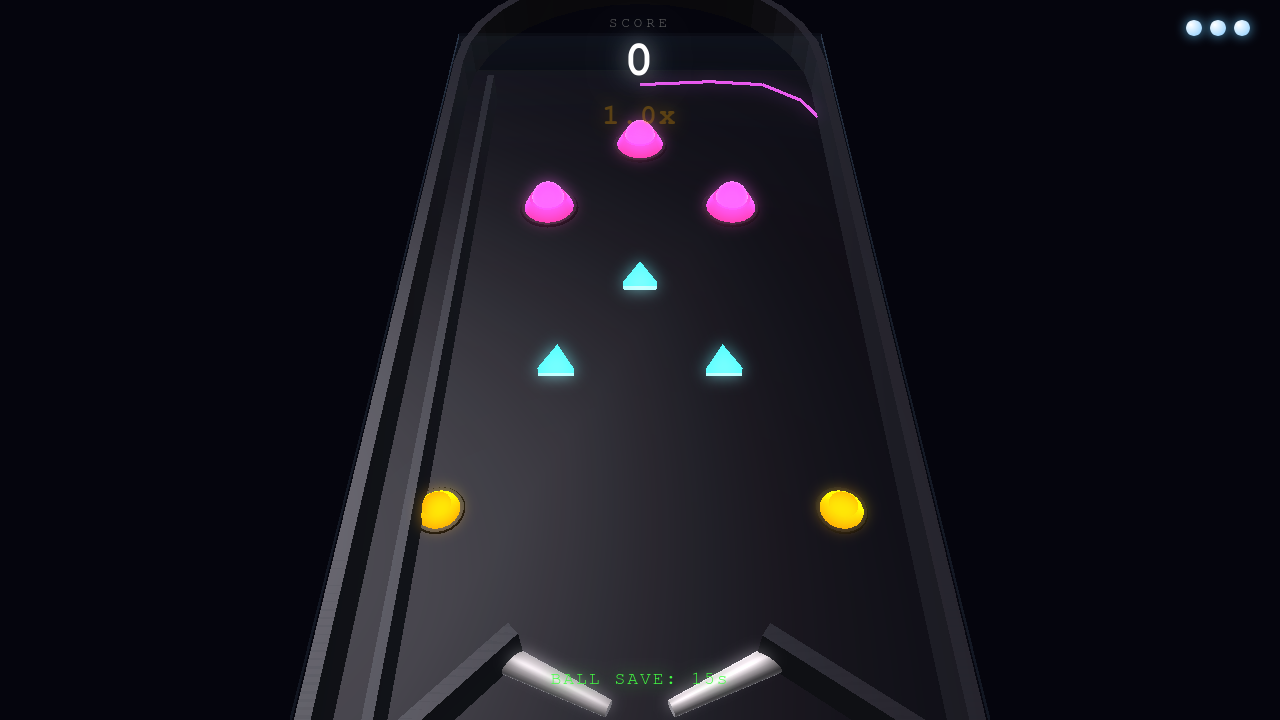
\includegraphics[width=\linewidth]{figures/3d-pinball.png}
    \captionof{figure}{3D Pinball: hand-rolled 2D physics on a tilted table, a PBR metal
    ball with cubemap reflection, Bloom post-processing, and Web Audio SFX. Awards 10
    tokens on game over.}
  \end{minipage}\hfill
  \begin{minipage}{0.48\textwidth}
    \centering
    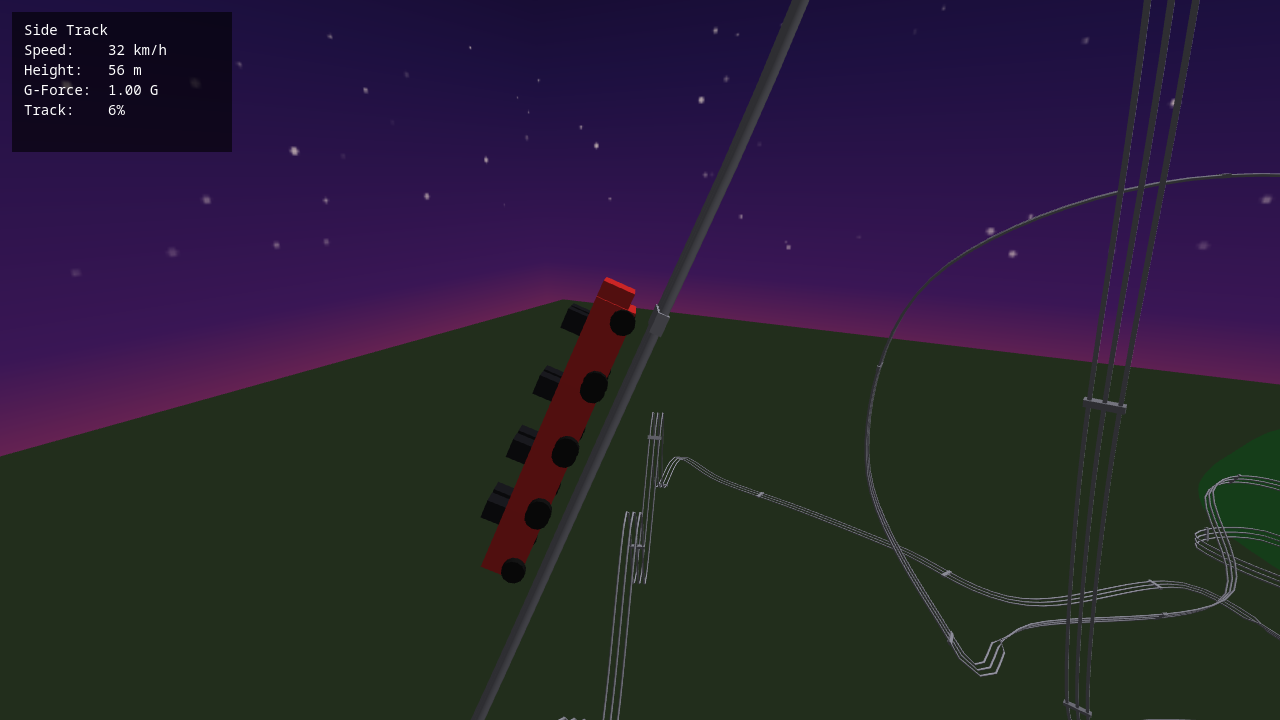
\includegraphics[width=\linewidth]{figures/roller-coaster.png}
    \captionof{figure}{Roller Coaster: Catmull-Rom spline track with Frenet--Serret (TNB)
    frame orientation, energy-conservation physics, and a 2D-canvas HUD (speed / height /
    G-force / progress). Consumes 10 tokens per ride.}
  \end{minipage}
\end{figure}

\begin{figure}[H]
  \centering
  \begin{minipage}{0.48\textwidth}
    \centering
    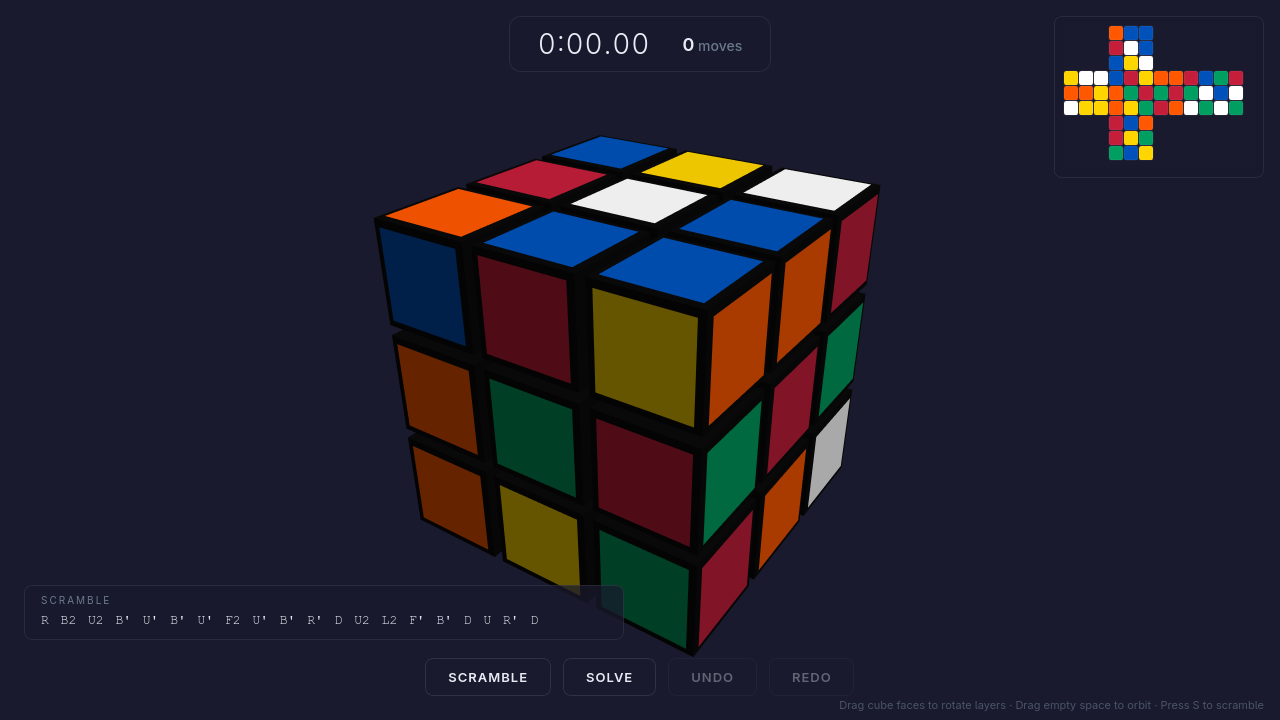
\includegraphics[width=\linewidth]{figures/rubiks-cube.png}
    \captionof{figure}{Rubik's Cube: raycast face-picking, drag-to-rotate with
    \texttt{easeOutBack} snap, a layer-by-layer auto-solver, and a live 2D cross-net.
    Awards 10 tokens on solve.}
  \end{minipage}\hfill
  \begin{minipage}{0.48\textwidth}
    \centering
    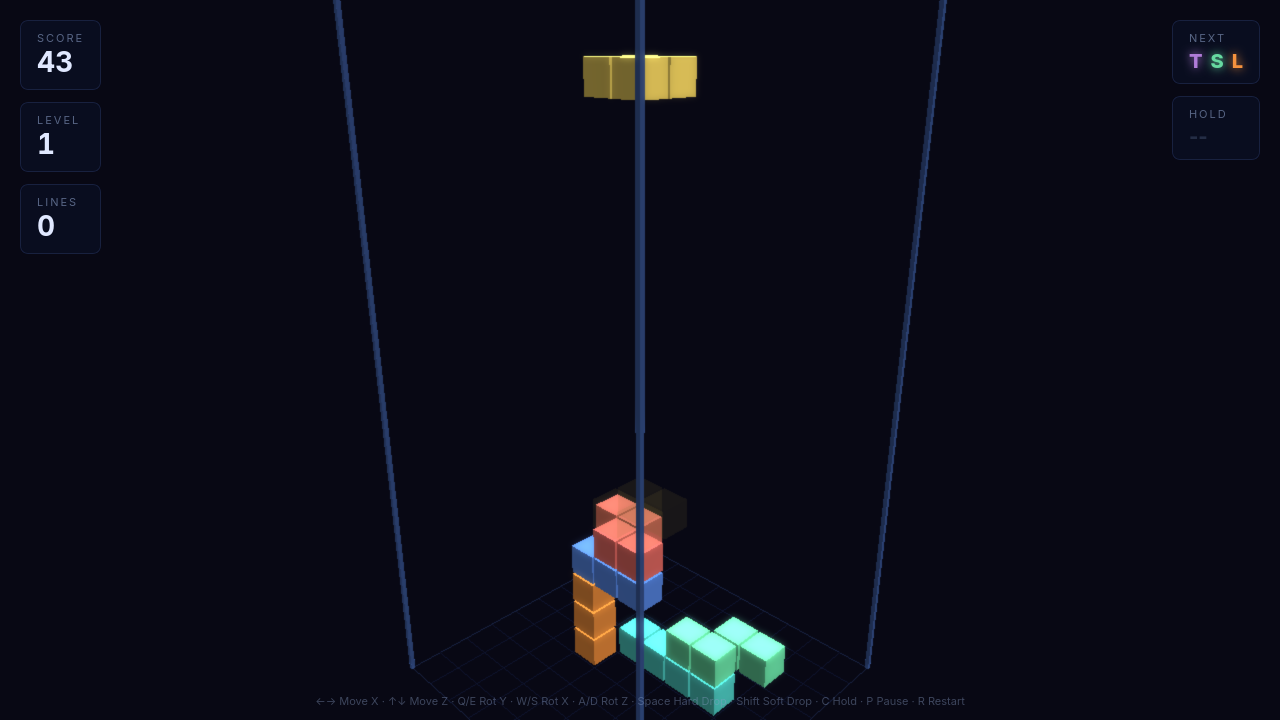
\includegraphics[width=\linewidth]{figures/3d-tetris.png}
    \captionof{figure}{3D Tetris: a $10\!\times\!20\!\times\!10$ volumetric well with
    SDF round-edge blocks, three-axis rotation (wall-kick corrected), ghost-piece
    preview, Bloom post-processing, and a grey-scale game-over fade. Awards 10 tokens
    on game over.}
  \end{minipage}
\end{figure}

% =====================================================================
\section{Challenges and Solutions}

\subsection{The Skybox Was Invisible: the \texttt{mat3 + xyww} Trap}

\textbf{Symptom.} The skybox mesh ($500^3$ box, cubemap texture) was completely invisible.
Changing the fragment shader to output pure red produced no red pixels. No WebGL errors.

\textbf{Root cause.} The textbook skybox trick uses
\texttt{gl\_Position = (projection * mat3(modelView) * pos).xyww} to force $z = w$ so the
box sits on the far plane. The \texttt{mat3()} strips translation; \texttt{xyww} forces
depth. This assumes the camera is at the box centre. In our walkthrough scene the camera is
at \texttt{[0, 1.7, 18]}, \emph{not} at the origin. For vertices behind the camera (e.g.\
the $+Z$ face at view-space $z = 250$), the post-projection $w$ is negative, and the
\texttt{xyww} trick sets $z = w < 0$. The clip test $-w \le z \le w$ then becomes
``positive $\le$ negative $\le$ negative'', which fails. Roughly half the box's vertices
were clipped away, collapsing most triangles.

\textbf{Fix.} Abandon the \texttt{mat3/xyww} trick entirely. Use standard projection
(\texttt{gl\_Position = projection * modelView * vec4(pos,1)}) with a physically giant box
($500^3$) centred at the world origin so the camera is always inside it. Render with
\texttt{cullFace = GL\_FRONT}, \texttt{depthWrite = false}, and
\texttt{frustumCulled = false}. This is robust for any camera position.

\subsection{OGL Array-Uniform Naming}

\textbf{Symptom.} With \texttt{uniform vec3 uLightPos[8]} in the shader, OGL logged
``Active uniform uLightPos[0] has not been supplied'' every frame, even though we passed
values.

\textbf{Root cause.} OGL's \texttt{Program} parses the active-uniform name
\texttt{uLightPos[0]} with a regex and looks up \texttt{this.uniforms['uLightPos']}. If
the uniforms object was keyed as \texttt{'uLightPos[0]'} (as a naive port from raw
WebGL would do), the lookup misses. Separately, OGL's \texttt{flatten()} checks
\texttt{Array.isArray(value)}; a \texttt{Float32Array} returns \texttt{false} and is
misinterpreted as a struct.

\textbf{Fix.} (1) Key uniforms by the base name only (\texttt{uLightPos}, not
\texttt{uLightPos[0]}). (2) Pass a plain JavaScript \texttt{Array} (not
\texttt{Float32Array}) as the value. OGL then flattens and uploads via
\texttt{uniform3fv} correctly.

\subsection{ES-Module Import Paths and the \texttt{miniserve} Symlink}

\textbf{Symptom.} \texttt{import \{\ldots\} from '../../ogl/src/index.js'} 404'd when the
server root was the \texttt{Theme-Park/} directory, because the browser normalised the
relative path back to the server root where \texttt{ogl/} did not exist.

\textbf{Fix.} Serve from the \emph{repo root} (so all sibling game directories resolve),
and add a \texttt{Theme-Park/ogl -> ../ogl} symlink so that the \texttt{../../ogl/...}
path also resolves when \texttt{Theme-Park/} is served alone. \texttt{miniserve} must not
be passed \texttt{-{}-no-symlinks}.

% =====================================================================
\section{Most Proud Of}

What we are most proud of is not any single technique but the \textbf{project's
trajectory}. The four sub-games did not start as components of a theme park---they began
as independent experiments. While learning the OGL library we built each game in
isolation: a neon Pinball table to push hand-rolled physics and PBR metal, a Rubik's Cube
to solve quaternion layer-rotation and raycast face-picking, a 3D Tetris to exercise
SDF shaders and Bloom post-processing, and a Roller Coaster to tackle Catmull-Rom
splines and Frenet--Serret framing. Each was a self-contained playground that explored a
different corner of real-time computer graphics.

The insight that turned four demos into one game was the \textbf{theme-park hub}. Instead
of discarding the prototypes or rewriting them into a single renderer (an engineering
nightmare with four independent OGL scenes), we asked: what if the park itself \emph{is}
the integration layer? A first-person plaza where each door leads to a different game
universe, connected by a shared token economy and a persistent save state. The hub then
becomes the single place where every hard graphics requirement---skybox, Phong point
lights, shadow mapping, cubemap reflection, textured surfaces, camera control---is
concentrated and shown off at dusk, the one lighting condition where they all read
simultaneously.

So the real achievement is the \emph{architecture}: the four games kept their original
physics, rendering, and gameplay untouched, and the hub glued them together with nothing
more than page navigation, \texttt{localStorage}, and a shared hooks module. What was
originally ``four ways to explore a library'' became \emph{Dusk Park}---one cohesive game
where the player earns tokens in an arcade, spends them on a coaster ride, and watches
fireworks after three tours, all set against a dusk sky that makes every graphics
technique visible in a single frame.

\end{document}
